\documentclass[aspectratio=169]{beamer}

% Pacotes essenciais
\usepackage[utf8]{inputenc}
\usepackage[T1]{fontenc}
\usepackage[brazilian]{babel}
\usepackage{graphicx}
\usepackage{tikz}

% Fonte moderna Roboto
\usepackage[sfdefault]{roboto}
\usepackage[T1]{fontenc}

% Definição das cores
\definecolor{vermelhoPrincipal}{HTML}{b11116}
\definecolor{azulComplementar}{HTML}{3a5461}
\definecolor{brancoFundo}{HTML}{FFFFFF}

% Configuração do tema
\usetheme{Madrid}
\usecolortheme{default}

% Cores personalizadas - texto sempre em preto
\setbeamercolor{structure}{fg=black}
\setbeamercolor{palette primary}{bg=vermelhoPrincipal,fg=white}
\setbeamercolor{palette secondary}{bg=azulComplementar,fg=white}
\setbeamercolor{palette tertiary}{bg=vermelhoPrincipal,fg=white}
\setbeamercolor{palette quaternary}{bg=azulComplementar,fg=white}
\setbeamercolor{frametitle}{bg=vermelhoPrincipal,fg=white}
\setbeamercolor{background canvas}{bg=brancoFundo}
\setbeamercolor{title}{fg=black}
\setbeamercolor{subtitle}{fg=azulComplementar}
\setbeamercolor{author}{fg=black}
\setbeamercolor{date}{fg=black}
\setbeamercolor{itemize item}{fg=black}
\setbeamercolor{itemize subitem}{fg=black}
\setbeamercolor{enumerate item}{fg=black}
\setbeamercolor{block title}{bg=vermelhoPrincipal,fg=white}
\setbeamercolor{block body}{bg=vermelhoPrincipal!10,fg=black}
\setbeamercolor{normal text}{fg=black}

% Configurar fonte dos itemize
\setbeamerfont{itemize/enumerate body}{size=\scriptsize}
\setbeamerfont{itemize/enumerate subbody}{size=\scriptsize}

% Marcadores modernos e minimalistas
\setbeamertemplate{itemize item}{\raisebox{0.2ex}{\rule{0.6ex}{0.6ex}}}
\setbeamertemplate{itemize subitem}{\raisebox{0.3ex}{\rule{0.4ex}{0.4ex}}}
\setbeamertemplate{itemize subsubitem}{\raisebox{0.35ex}{\rule{0.3ex}{0.3ex}}}
\setbeamertemplate{enumerate items}[square]

% Transições suaves
\setbeamercovered{transparent}

% Remover símbolos de navegação
\setbeamertemplate{navigation symbols}{}

% Customizar o cabeçalho com barra vermelha e logo
\setbeamertemplate{headline}{
  \begin{beamercolorbox}[wd=\paperwidth,ht=0.6cm,dp=0.15cm,leftskip=0.2cm,rightskip=0.4cm]{palette primary}
    \raisebox{-0.05cm}{
\includegraphics[height=0.45cm]{imgs/base/fatec-rgt.png}}
    \hfill
    \raisebox{-0.18cm}{
\includegraphics[height=0.85cm]{imgs/base/governo-sp-secretaria-logo.png}}
    \hspace{0.2cm}
    \raisebox{-0.08cm}{
\includegraphics[height=0.6cm]{imgs/base/cps-logo.png}}
  \end{beamercolorbox}
}
% Remover sombras dos blocks
\setbeamertemplate{blocks}[default]
\setbeamertemplate{itemize/enumerate body begin}{\scriptsize}
\setbeamertemplate{itemize/enumerate subbody begin}{\scriptsize}
% Customizar o rodapé
\setbeamertemplate{footline}{
  \begin{beamercolorbox}[wd=\paperwidth,ht=0.4cm,dp=0.2cm,leftskip=0.3cm,rightskip=0.3cm]{palette secondary}
    \usebeamerfont{footline}
    \insertshortauthor \hfill \hfill {\fontsize{5}{6}\selectfont\insertshorttitle} \hfill \hfill \insertframenumber/\inserttotalframenumber
  \end{beamercolorbox}
}

% Customizar título do frame
\setbeamertemplate{frametitle}{
  \vspace{0.3cm}
  \textcolor{black}{\insertframetitle}
  \vspace{0.1cm}
}

% Informações da apresentação
\title{Sistema para Identificação a Pinta Preta na Tangerina \\Ponkan, orientado por Visão Computacional}
\subtitle{}
\author[DSM]{PARRA, A.; FIEL, D.; PEREIRA, G.; KLETELINGER, G.; OLIVEIRA, M.}
\institute{Desenvolvimento de Software Multiplataforma\\FATEC Registro}
\date{\today}

\begin{document}

% Slide de título moderno
\begin{frame}
  \vspace{0.8cm}
  \begin{center}
    \begin{tikzpicture}
      % Linha decorativa superior
      \draw[vermelhoPrincipal, line width=2pt] (-4,0) -- (4,0);
    \end{tikzpicture}
    
    \vspace{0.4cm}
    
    {\normalsize\bfseries\inserttitle}\par
    
    \vspace{0.2cm}
    
    {\tiny\insertauthor}\par
    
    \vspace{0.1cm}
    
    {\small\textcolor{azulComplementar}{\insertsubtitle}}\par
    
    \vspace{0.5cm}
    
    \begin{tikzpicture}
      % Linha decorativa inferior
      \draw[azulComplementar, line width=1.5pt] (-2.5,0) -- (2.5,0);
    \end{tikzpicture}
    
    \vspace{0.3cm}
    
    {\scriptsize\insertinstitute}\par
    
    \vspace{0.01cm}
    
    {\tiny\textcolor{azulComplementar}{\insertdate}}\par
  \end{center}
\end{frame}

% Slide de agenda
\begin{frame}[b]{Agenda}
  \begin{itemize}
    \item Pitch
    \item Problematização
    \item Objetivo
    \item Estado da Arte
    \item Ferramental
    \item Metodologia
    \item Apresentação prática
  \end{itemize}
  
  \vfill
  
  \hfill{\scriptsize \textbf{Duração:} 10 a 11 min.}
\end{frame}

\section{Pitch}
{
\usebackgroundtemplate{%
  
\includegraphics[width=\paperwidth,height=\paperheight]{imgs/wallpaper.jpg}%
}
\begin{frame}[b]{Pitch}

\vspace*{\fill}

\begin{center}

  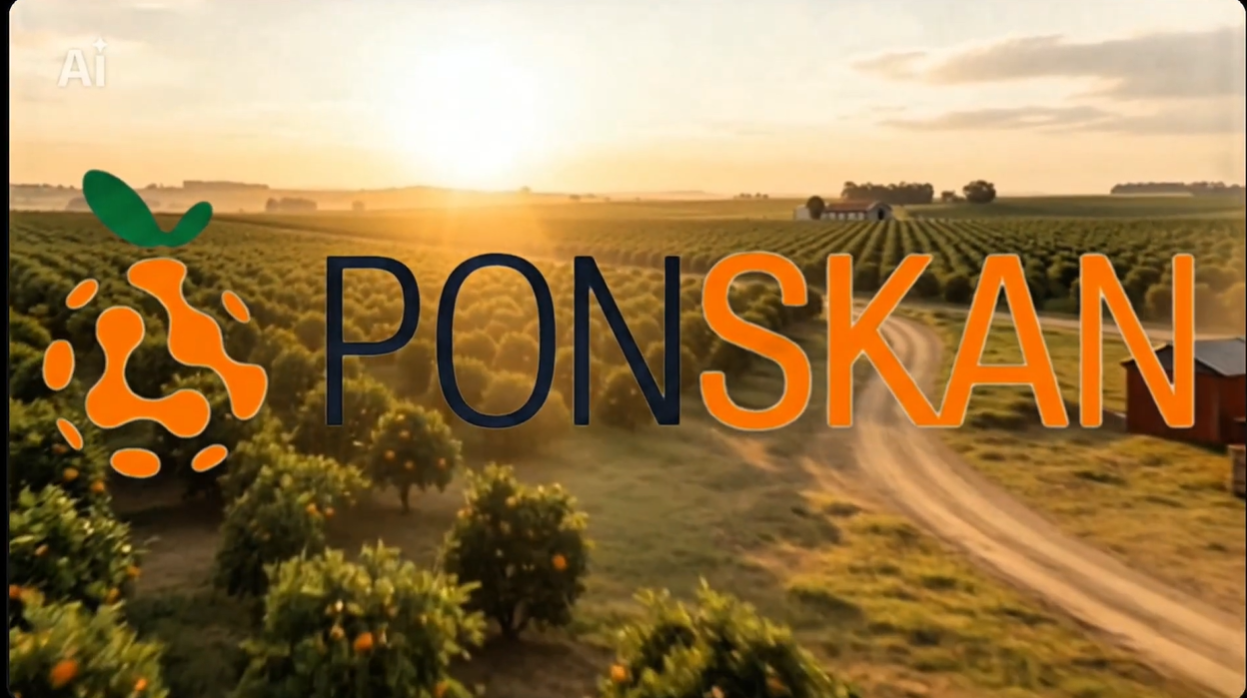
\includegraphics[width=4cm, height=2cm]{imgs/thumb.png}

  \vspace{1cm}

  Clique \href{https://www.youtube.com/watch?v=Qy9XhNMbdHU}{aqui} para assistir.
\end{center}

\vspace*{\fill}

  % \begin{itemize}
  %   \item \parbox{0.60\textwidth}{Apresentação concisa e objetiva do projeto}
  %   \item \parbox{0.60\textwidth}{Destaque do \textbf{problema} que o projeto resolve}
  %   \item \parbox{0.60\textwidth}{Proposta de \textbf{valor} e diferenciais da solução}
  %   \item \parbox{0.60\textwidth}{Público-alvo e \textbf{impacto} esperado}
  %   \item \parbox{0.60\textwidth}{Visão geral das \textbf{tecnologias} utilizadas}
  % \end{itemize}
  
  % \vfill
  
  {\fontsize{4}{5}\selectfont\hfill\textcolor{white}{Imagem: gerada por Gemini}}
\end{frame}
}

\section{Problematização}

{
\usebackgroundtemplate{%
  
\includegraphics[width=\paperwidth,height=\paperheight]{imgs/wallpaper.jpg}%
}
\begin{frame}[b]{Problematização}
  \begin{itemize}
    \item \parbox{0.65\textwidth}{Brasil é o \textbf{maior produtor} de laranja do mundo \break (aprox. \textcolor{orange}{\textbf{75\%}} das exportações mundiais de suco)}
    \break
    \item \parbox{0.65\textwidth}{Citricultura é essencial para \textbf{agricultura familiar} \break (\textcolor{orange}{\textbf{+60\%}} dos estabelecimentos agrícolas do Vale do Ribeira)} 
    \break
    \item \parbox{0.65\textwidth}{\textbf{Pinta Preta} diminui produtividade pois causa quedas prematuras e manchas}
    \item \parbox{0.65\textwidth}{Inspeção manual da doença ainda é \textbf{difícil} e \textbf{subjetiva}}
    \item \parbox{0.65\textwidth}{Pequenos produtores não possuem \textbf{acesso adequado} à tecnologia}
    \item \parbox{0.65\textwidth}{\textbf{Clima quente e úmido} da região favorece o desenvolvimento do fungo}
  \end{itemize}
  
  \vfill
  
  {\fontsize{4}{5}\selectfont\textit{Fonte: USDA (2025), IBGE (2017)}\hfill\textcolor{white}{Imagem: gerada por Gemini}}
\end{frame}
}

\section{Objetivo}

{
\usebackgroundtemplate{%
  
\includegraphics[width=\paperwidth,height=\paperheight]{imgs/wallpaper.jpg}%
}
\begin{frame}[b]{Objetivo}
  \begin{itemize}
    \item \parbox{0.60\textwidth}{\textbf{Objetivo geral}: desenvolver sistema para detectar pinta preta em tangerinas usando técnicas de visão computacional}
    \item \parbox{0.60\textwidth}{\textbf{Objetivos específicos}:}
    \begin{itemize}
      \item \parbox{0.55\textwidth}{Emitir recomendações de manejo personalizadas consultando \textcolor{orange}{\textbf{dados climáticos}}}
      \item \parbox{0.55\textwidth}{Gerar mapa dos pontos de infecção e áreas de risco do pomar usando \textcolor{orange}{\textbf{geolocalização}}}
    \end{itemize}
  \end{itemize}
  
  \vfill
  
  {\fontsize{4}{5}\selectfont\textit{Fonte: Autoria própria (2026)}\hfill\textcolor{white}{Imagem: gerada por Gemini}}
\end{frame}
}

\section{Estado da Arte}

\definecolor{verdeClaro}{RGB}{0,198,141}
\definecolor{azulEscuro}{RGB}{0,51,102}

\begin{frame}[t]{Estado da Arte}
  \scriptsize
  
  % Análise de \textbf{soluções existentes} no mercado, comparação de \textbf{tecnologias} e abordagens, identificação de \textbf{gaps} e oportunidades, referências bibliográficas e \textbf{trabalhos relacionados}, tendências e \textbf{inovações} na área.
  
  \vspace{0.3cm}
  
  \begin{table}
    \centering
    \tiny
    \begin{tabular}{|p{2.5cm}|p{2cm}|p{2cm}|p{2cm}|p{2cm}|p{1.5cm}|}
      \hline
      \textbf{Título/Autores} & \textbf{Objetivo} & \textbf{Método} & \textbf{Resultados} & \textbf{Limitações} & \textbf{Gap} \\
      \hline
      Diferenciação do Greening de Outras Doenças Foliares em Citros Utilizando Técnicas de Processamento de Imagens \textit{(Ribeiro; Castro Jorge; Paiva, 2012)} & Diferenciar greening de outras doenças em folhas de citros & Scanner, Segmentação de Cores, Descritores de Forma, RNA & \textcolor{red}{\textbf{43\%}} a \textcolor{red}{\textbf{63\%}} de acurácia na classificação global & Similaridade entre sintomas, Dataset restrito & Não integra dados de contorno + cor \\
      \hline
      Identificação de huanglongbing (hlb) em plantações de citros utilizando redes convolucionais profundas \textit{(Marques; Pontelli; Paiva, 2022)} & Identificar greening em folhas de citros utilizando CNN & Câmeras digitais \break Data augmentation \break Transfer Learning \break CNN & \textcolor{verdeClaro}{\textbf{95,99\%}} de acurácia em fundos reais & Necessidade de fine-tuning ocasionada pelo pré-treinamento usando ImageNet & Não considera a análise de frutos \\
      \hline
      Detection of citrus black spot disease and ripeness level in orange fruit using learning-to-augment incorporated deep networks \textit{(Momeny et al., 2022)} & Identificar blackspot e nível de maturação em laranjas & Câmeras digitais \break Diferentes modelos de CNN \break Learning to augment & \textcolor{verdeClaro}{\textbf{99,5\%}} de acurácia com ResNet50 & Risco de overfitting pela desproporção entre dataset e profundidade do ResNet50 & Não valida em outras variedades de citros \\
      \hline
    \end{tabular}
  \end{table}
\end{frame}

\section{Ferramental}

{
\usebackgroundtemplate{%
  
\includegraphics[width=\paperwidth,height=\paperheight]{imgs/wallpaper.jpg}%
}
\begin{frame}[b]{Ferramental}
  \begin{itemize}
    \item \parbox{0.60\textwidth}{\textbf{Linguagens}: JavaScript, Python}
    \item \parbox{0.60\textwidth}{\textbf{Frameworks e Bibliotecas}: React, Next, Node, Express, BullMQ, Sharp}
    \item \parbox{0.60\textwidth}{\textbf{Banco de dados}: MySQL, Redis}
    % \item \parbox{0.60\textwidth}{\textbf{Infraestrutura}: AWS, Docker, Kubernetes, etc}
    \item \parbox{0.60\textwidth}{\textbf{Ferramentas}: Git, GitHub, VS Code, Figma, Jira}
    % \item \parbox{0.60\textwidth}{\textbf{APIs} e integrações utilizadas}
  \end{itemize}
  
  \vfill
  
  {\fontsize{4}{5}\selectfont\textit{Fonte: Autoria própria (2026)}\hfill\textcolor{white}{Imagem: gerada por Gemini}}
\end{frame}
}

\section{Metodologia}

{
\usebackgroundtemplate{%
  % 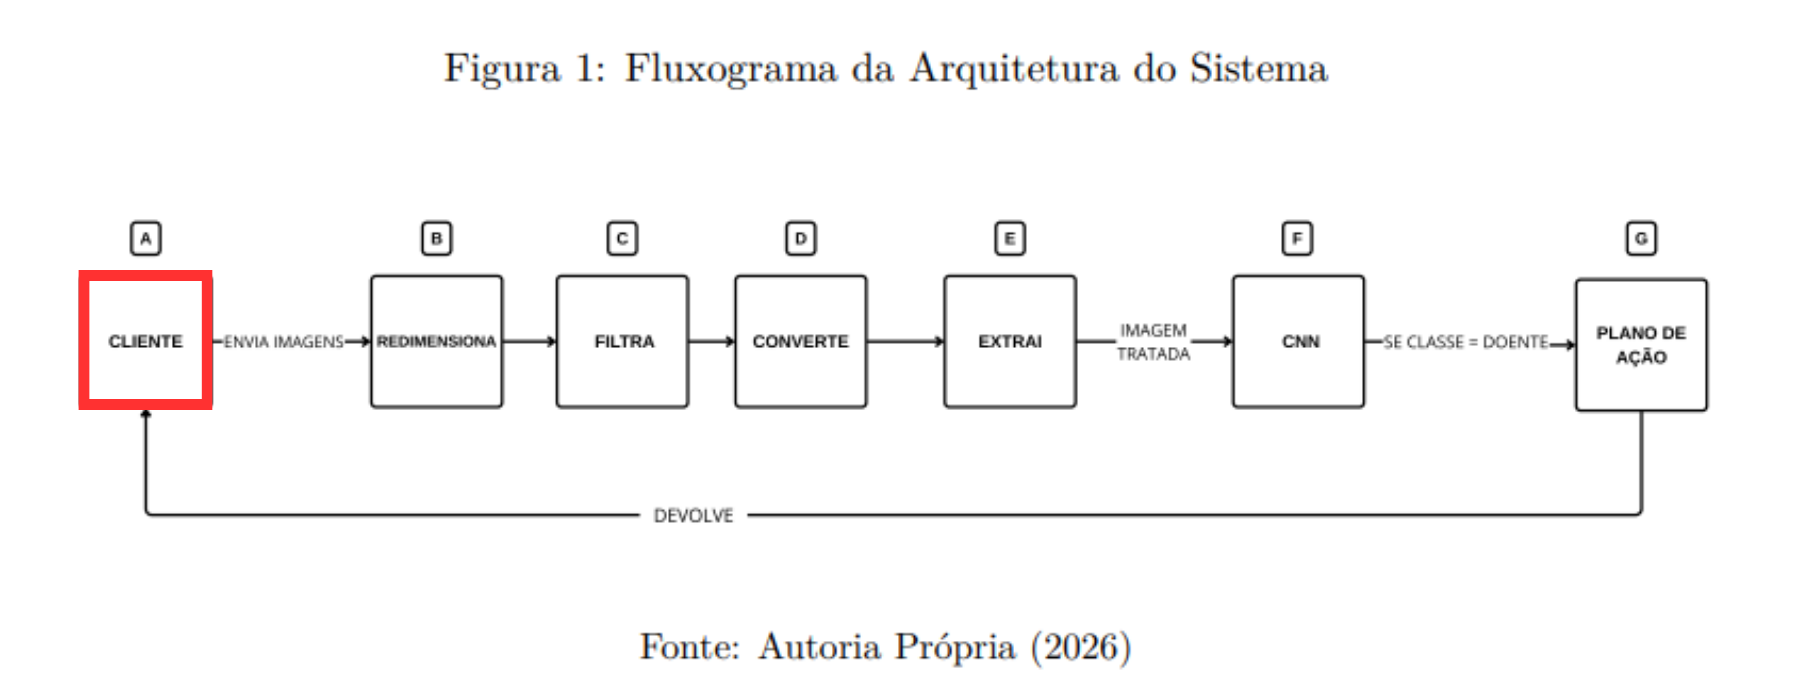
\includegraphics[width=15cm,height=8cm]{imgs/metodologia01.png}%
}
\begin{frame}[t]{Metodologia}

  \begin{center}
    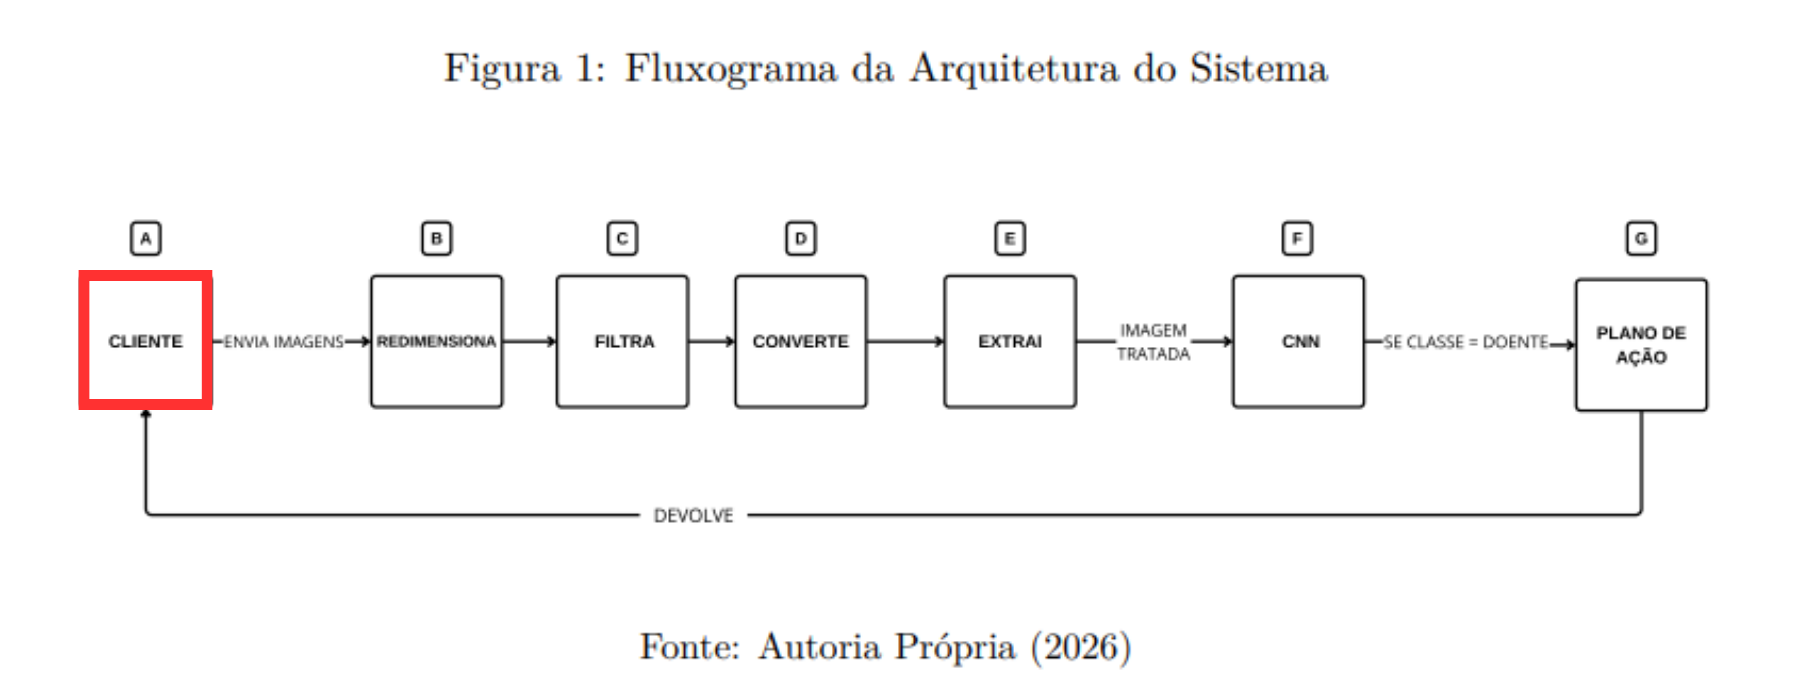
\includegraphics[width=10cm, height=4cm]{imgs/metodologia01.png}
  \end{center}
  
  \break
  
  \scriptsize 
  (A) O produtor rural captura de 1-4 imagens no app Web/Mobile. As imagens são enviadas para nossa API Rest.

  {\fontsize{4}{5}\selectfont\textit{Fonte: Autoria própria (2026)}}
\end{frame}

\begin{frame}[t]{Metodologia}

  \begin{center}
    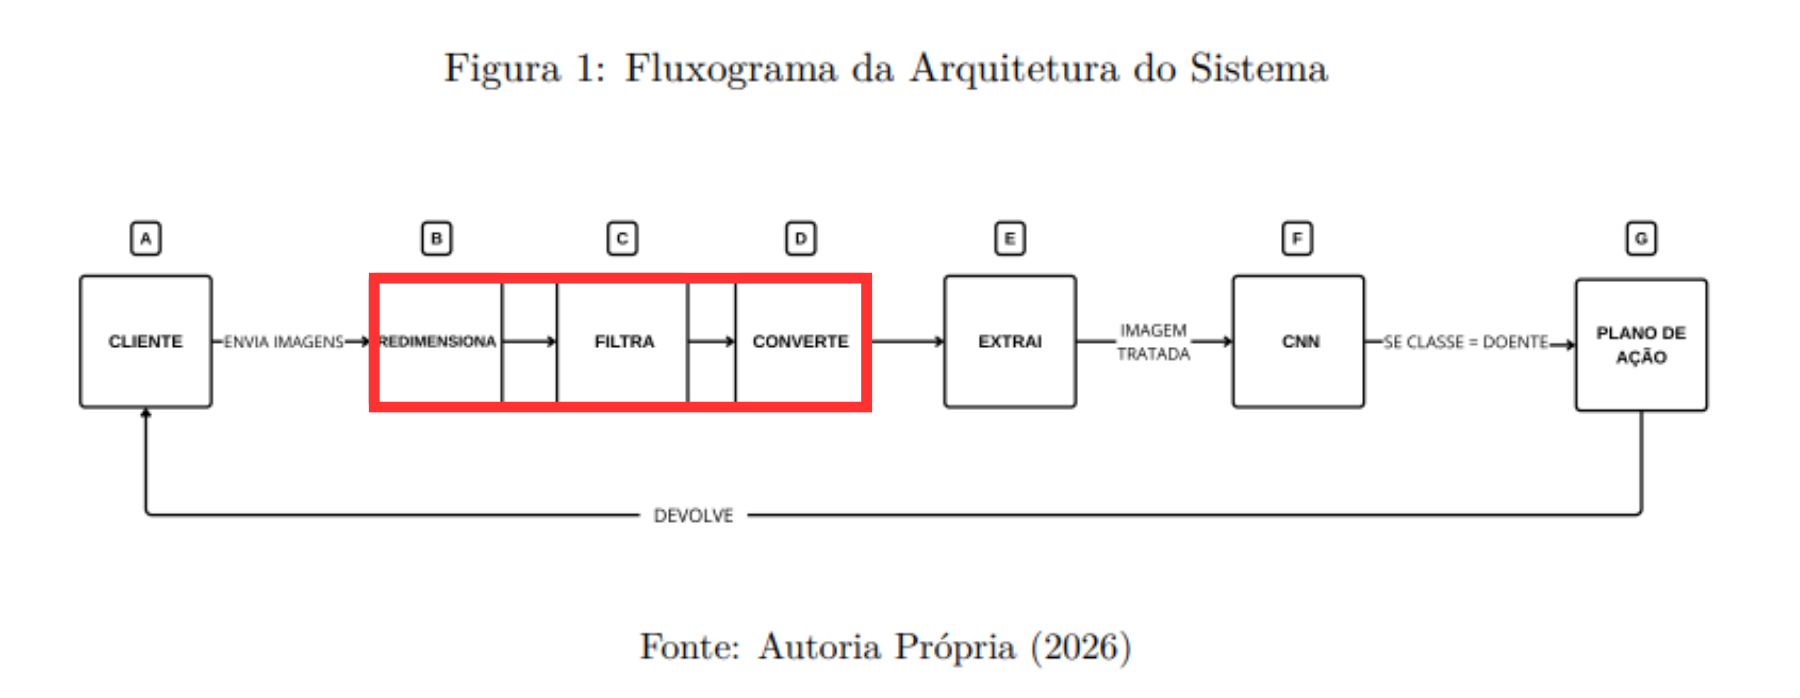
\includegraphics[width=10cm, height=4cm]{imgs/metodologia02.png}
  \end{center}
  
  \break
  
  \scriptsize 
  (B-D) Imagens são redimensionadas, filtradas e convertidas em buffer no padrão de cor “sRGB”, em uma fila assíncrona e paralela ao Node.js.

  {\fontsize{4}{5}\selectfont\textit{Fonte: Autoria própria (2026)}}
\end{frame}

\begin{frame}[t]{Metodologia}

  \begin{center}
    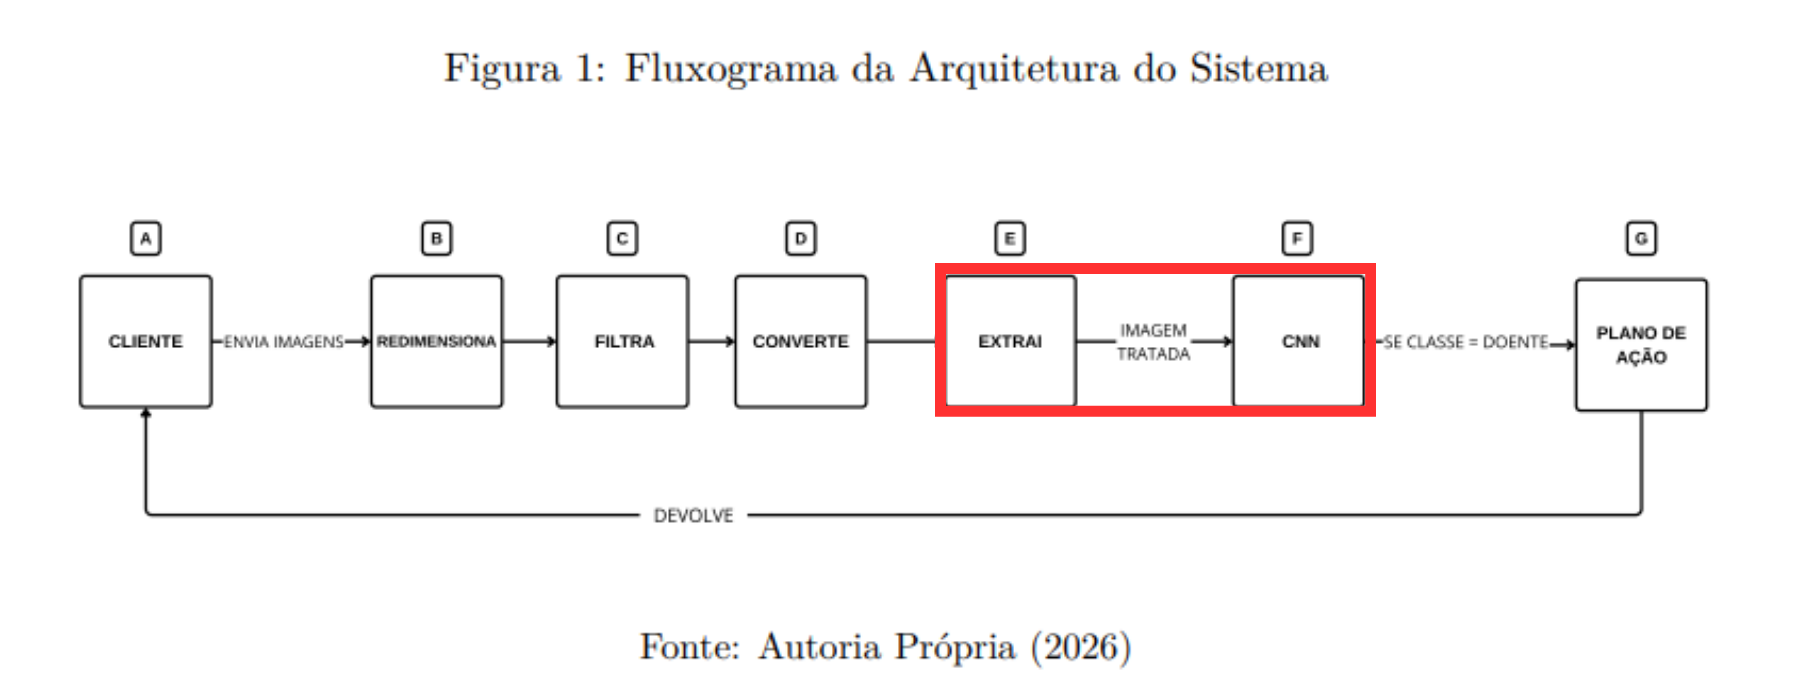
\includegraphics[width=10cm, height=4cm]{imgs/metodologia03.png}
  \end{center}
  
  \break
  
  \scriptsize 
  (E-F) Buffers são enviados para Fast API e classificados por modelo de CNN. Planejamos usar YOLO para segmentação e EfficientNet para classificação.

  {\fontsize{4}{5}\selectfont\textit{Fonte: Autoria própria (2026)}}
\end{frame}

\begin{frame}[t]{Metodologia}

  \begin{center}
    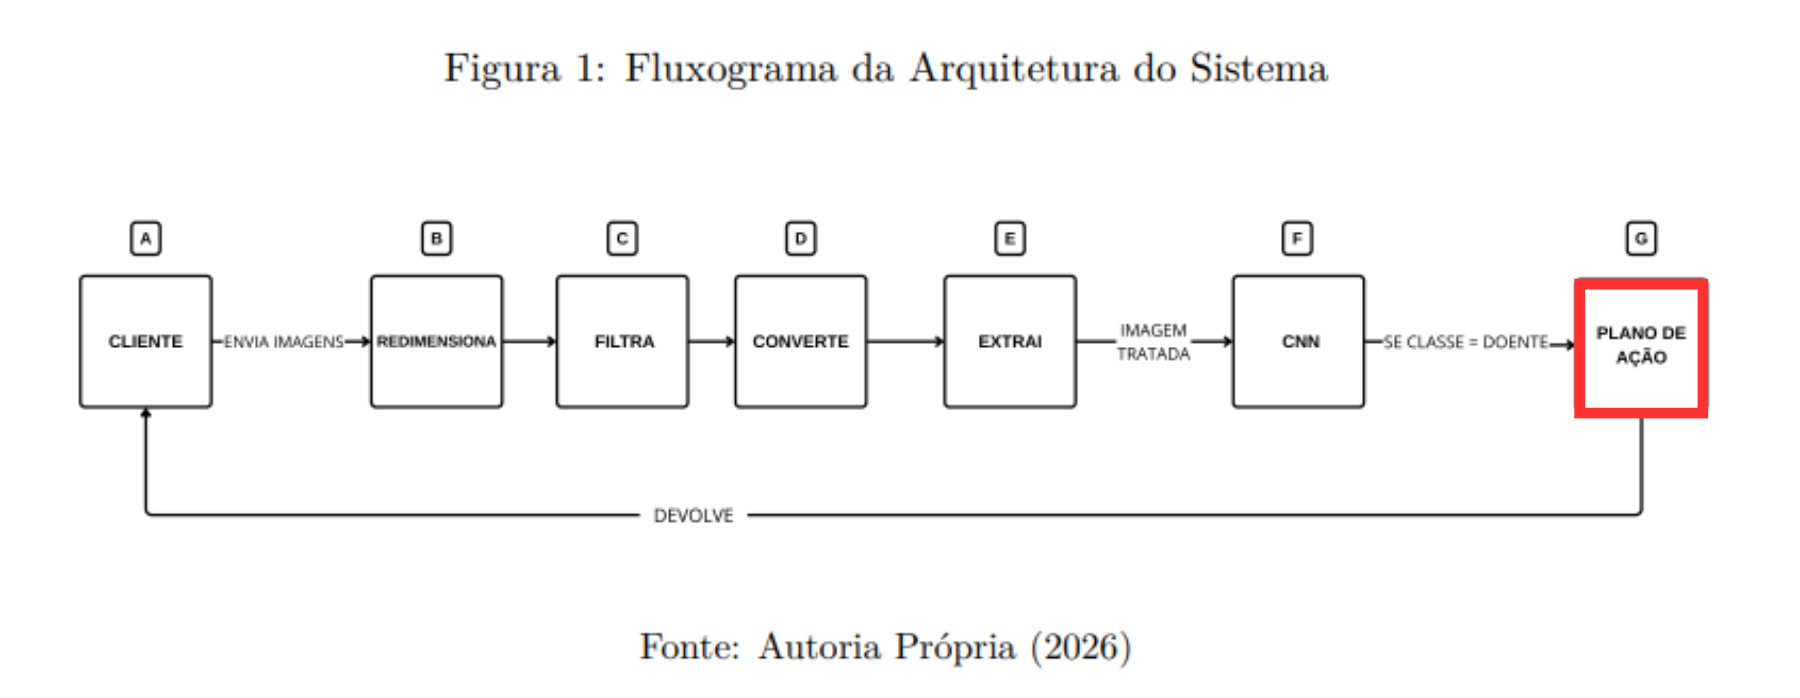
\includegraphics[width=10cm, height=4cm]{imgs/metodologia04.png}
  \end{center}
  
  \break
  
  \scriptsize 
  (G) Sistema constrói plano de ação com base no pré-diagnóstico, devolvendo os dados para a interface do cliente.

  {\fontsize{4}{5}\selectfont\textit{Fonte: Autoria própria (2026)}}
\end{frame}
}

\section{Apresentação Prática}

{
\usebackgroundtemplate{%
  
\includegraphics[width=\paperwidth,height=\paperheight]{imgs/wallpaper.jpg}%
}
\begin{frame}[b]{Apresentação Prática}
  \begin{itemize}
    \item \parbox{0.60\textwidth}{\textbf{Demonstração} ao vivo do sistema}
    \item \parbox{0.60\textwidth}{\textbf{Interface} e experiência do usuário}
    \item \parbox{0.60\textwidth}{Principal \textbf{funcionalidade} implementada: Fluxo da análise de amostras}
    
  \end{itemize}
  
  \vfill
  
  {\fontsize{4}{5}\selectfont\hfill\textcolor{white}{Imagem: gerada por Gemini}}
\end{frame}
}

% \section{Resultados e Discussões}

% {
% \usebackgroundtemplate{%
%   
\includegraphics[width=\paperwidth,height=\paperheight]{imgs/img_008.jpg}%
% }
% \begin{frame}[b]{Resultados e Discussões}
%   \begin{itemize}
%     \item \parbox{0.60\textwidth}{Principais \textbf{resultados} alcançados}
%     \item \parbox{0.60\textwidth}{Análise de \textbf{métricas} e indicadores}
%     \item \parbox{0.60\textwidth}{Feedback dos \textbf{usuários} e testes realizados}
%     \item \parbox{0.60\textwidth}{\textbf{Desafios} encontrados e soluções adotadas}
%     \item \parbox{0.60\textwidth}{Contribuições e \textbf{aprendizados} do projeto}
%     \item \parbox{0.60\textwidth}{\textbf{Trabalhos futuros} e melhorias propostas}
%   \end{itemize}
  
%   \vfill
  
%   {\fontsize{4}{5}\selectfont\textit{Fonte: Seu Nome}\hfill\textcolor{white}{Imagem: Descrição da imagem}}
% \end{frame}
% }

% Slide Informações Gerais (clone)
{
\usebackgroundtemplate{%
  
\includegraphics[width=\paperwidth,height=\paperheight]{imgs/wallpaper.jpg}%
}
\begin{frame}[b]{}
  \vspace{0.2cm}
  
  \hspace*{0.25\paperwidth}{\Large \textbf{Obrigado pela atenção!}}
  
  \vfill

  {\fontsize{4}{5}\selectfont\hfill\textcolor{white}{Imagem: gerada por Gemini}}
\end{frame}
}

\end{document}
